\documentclass[10pt,handout]{beamer}
\usetheme{Warsaw}
\usepackage[all]{xy}
\usepackage{comment}
\usepackage{verbatim}
\setbeamercovered{transparent}

%Italicised Theorems
\theoremstyle{plain}
\newtheorem{theo}{Theorem}[section]
\newtheorem*{theo*}{Theorem}
\newtheorem{prop}[theo]{Proposition}
\newtheorem{nprop}[theo]{Non-Proposition}
\newtheorem{lem}[theo]{Lemma}
\newtheorem{cor}[theo]{Corollary}
\newtheorem{claim}[theo]{Claim}
\newtheorem{conj}[theo]{Conjecture}

%Roman Script Theorems
\theoremstyle{definition}
\newtheorem{defin}[theo]{Definition}
\newtheorem{nondefin}[theo]{Non-definition}
\newtheorem*{rem*}{Remark}
\newtheorem{rem}[theo]{Remark}
\newtheorem{rems}[theo]{Remarks}

%Math Operators
\DeclareMathOperator{\id}{id}
\DeclareMathOperator{\im}{im}
\DeclareMathOperator{\cod}{cod}
\DeclareMathOperator{\dom}{dom}
\DeclareMathOperator{\comp}{comp}
\DeclareMathOperator{\hset}{Hom}
\DeclareMathOperator{\Ob}{Ob}
\DeclareMathOperator{\Or}{o}
\DeclareMathOperator{\Ar}{Ar}
\DeclareMathOperator{\coker}{coker}
\DeclareMathOperator{\fr}{Rank}
\DeclareMathOperator{\subob}{Subob}
\DeclareMathOperator{\gr}{gr}
\DeclareMathOperator{\SA}{SA}

%New commands
\newcommand{\cupdot}{\mathbin{\mathaccent\cdot\cup}}
\newcommand\A{\mathcal{A}}
\newcommand\B{\mathcal{B}}
\newcommand\Cb{\mathcal{C}}
\newcommand\C{\mathbb{C}}
\newcommand\HQ{\mathbb{H}}
\newcommand\Z{\mathbb{Z}}
\newcommand\Q{\mathbb{Q}}
\newcommand\R{\mathbb{R}}
\newcommand\N{\mathbb{N}}
\newcommand\K{\mathbb{K}}
\newcommand\cat{\mathbf{C}}
\newcommand\catt{\mathbf{D}}
\newcommand\gen{\mathrm{GL}_n}
\newcommand\tplus{\>\widetilde{\oplus}\>}
\newcommand\ttimes{\>\widetilde{\otimes}\>}
\newcommand\tminus{\>\widetilde{\ominus}\>}
\newcommand\Tplus{\widetilde\oplus}
\newcommand\Ttimes{\widetilde\otimes}
\newcommand\Tminus{\widetilde\ominus}
\newcommand\wplus{\>\widehat{\oplus}\>}
\newcommand\Wplus{\widehat{\oplus}}
\newcommand\bplus{\>\bar{\oplus}\>}
\newcommand\Bplus{\bar{\oplus}}
\newcommand\Ef{\mathcal{E}}
\newcommand\MVEA{\mathbf{MVEA}}
\newcommand\BA{\mathbf{BA}}
\newcommand\EA{\mathbf{EA}}
\newcommand\MV{\mathbf{MV}}
\newcommand\BCM{\mathbf{BCM}}
\newcommand\catj{\mathbf{J}}
\newcommand\Pee{\mathcal{P}a}
\newcommand\Tee{\mathcal{T}o}
\newcommand\Em{\mathcal{M}}
\newcommand\Eye{\mathcal{I}}
\newcommand\Dee{\mathcal{D}}
\newcommand\Jay{\mathcal{J}}

\title{Formally certified code obfuscation \\ in the Coq proof assistant}

\author{Weiyun Lu \\ University of Ottawa}


\begin{document}

\begin{frame}[plain] %title
  \titlepage
\end{frame}

%\begin{frame}<0>{Why more than two truth values?}
%   Finite examples:
 % \begin{examples}
  %  \begin{enumerate}
  %  \item
 %       Aristotle: ``There will be a sea battle tomorrow".  Might depend on whether a storm occurs tomorrow.  Need at least third truth value.
%    \pause \item
%        Ulam's game of twenty questions:  fix a search space $S$ (a set of numbers).  Player A picks some $x_0 \in S$.  Player B has to guess $x_0$ by asking only yes or no questions. \pause
%        \par If Player A cannot lie, corresponds to usual 2-valued logic.  If Player A can lie $n-2$ times, then we have $n$ truth values.
%    \end{enumerate}\pause
%    Infinite examples (truth values in $[0,1]$):
%    \begin{enumerate}
%    \item
%        Probability of truth: ``It will rain tomorrow." \par
%    \item \par \pause
%        Degree of truth: ``People in this room like Justin Trudeau more than Stephen Harper."
%    \item \par \pause
%        Quantum stuff.
%  \end{enumerate}
%\end{examples}

%\end{frame}

\begin{frame}{Outline} %1

Part I: Background
\begin{itemize}
	\item Coq and formal verification.
	\item Code obfuscation.
	\item The IMP language.
\end{itemize}
\par\medskip
Part II: Contributions
\begin{itemize}
    \item Opaque predicate transformations.
    \item Control flow flattening: Smashing IFs.
    \item Control flow flattening: Smashing Whiles.
\end{itemize}

\end{frame}

\begin{frame}{What is Coq?} %2
\begin{center}
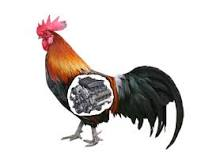
\includegraphics[scale=0.4]{coq}
\end{center}
Coq is:
\begin{itemize}\pause
    \item Le mot fran\c{c}ais pour ``rooster".
    \item An interactive theorem prover and functional programming language. \pause
    \item Think ``math textbook meets Lisp/Scheme''. \pause
    \item Provides formal methods, useful for both math and CS.
\end{itemize} \medskip
(Demo of {\color{red}DeMorgan} predicate logic proof.)
\end{frame}

\begin{frame}{The problem with informal methods in CS}
Why use Coq in software development?
\begin{itemize}
    \item Think ``super testing''.  Normal software testing is a bunch of ad-hoc examples; doesn't really show something is always correct; at best you show ``in these particular cases, these particular things that could go horribly wrong don't." \pause
    \item With formal verification, can specify statements with universal and existential quantifiers and prove them correct, i.e. ``For all ..., there exists ..., such that ...''.  Prove it will \emph{always} work / \emph{never} fail.  \pause
    \item In applied software engineering land, often times the definitions are murky and the numbers are made up.  ``5" and ``infinite" are practically the same thing.  Until they're not, of course. \pause
    \item Tradeoff: extremely high level of assurance that the thing does what it says on the box, but takes a lot of manpower/work.
    \item Best use cases: (parts of) code that are not overly complex, but where correctness is mission-critical.
\end{itemize}
\end{frame}

\begin{comment}
\begin{frame}{``If only they'd used formal verification..."} %3


\begin{center}
 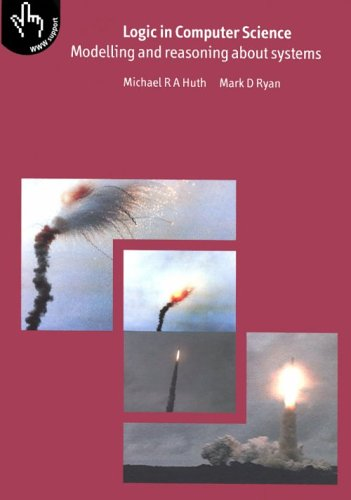
\includegraphics[scale=0.17]{ariane}  \par
 The Ariane 5 rocket:
 \begin{itemize}
 	\item Took a decade and \$ 7 billion to develop. \pause
 	\item Lifted off on June 4, 1996... \pause 
    \item ... and exploded 40 seconds later ... \pause
    \item ... because of one (superfluous!) line of code attempting to cast a 64-bit float to a 16-bit int ... \pause
    \item ... causing an exception which defaulted the tilt to a diagnostic value and caused an emergency shutdown in the onboard computers ... \pause
    \item ... a bug that would not have survived rigorous formal verification
 \end{itemize}
\end{center}
\end{frame}
\end{comment}

\begin{frame}{CompCert verified C compiler}
    Compilers turn source code (what a human reads and writes) into machine code (low-level instructions actually executed by the machine).  This is prone to errors.
    \par\medskip\pause
    CompCert is:
    \begin{itemize}
        \item Projected started by Xavier Leroy (ANR/INRIA, France) in 2005.
        \item Compiler for C, a notoriously buggy and unsafe language, that is specified, programmed, and proved correct in Coq.\pause
        \item 120000 lines of code since I last checked (summer 2017) and counting.
        \item Performance shown to be within a factor of 2 of non-verified counterparts.\pause
        \item Commercially available, used in mission critical software where high assurance that compiler preserves semantics is required.
    \end{itemize}
\end{frame}

\begin{comment}
\begin{frame}{Four-color theorem proved in Coq}
\begin{center}
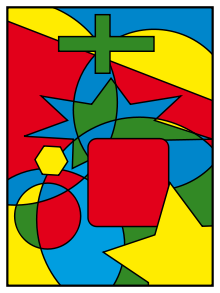
\includegraphics[scale=0.25]{fourcolortheorem}
\end{center}
\begin{theo}[Four-color theorem (graph theory)]
	Given any separation of a plane into contiguous regions, producing a figure called a map, no more than four colors are required to color the regions of the map so that no two adjacent regions have the same color.
\end{theo}
\begin{itemize}
	\item Conjectured in 1852. Many (incorrect) attempted proofs since.  Proven for five colors in 1890. \pause
    \item First proof with computer assistance in the 1980s, but would still require an infeasible amount of checking details by hand. \pause
    \item Finally, formal proof completed by a team led by Georges Gonthier at Microsoft in 2005.  No need to trust anything but Coq kernel.  The heavens part and angels sing.
\end{itemize}
\end{frame}
\end{comment}

\begin{comment}
\begin{frame}{Homotopy Type Theory}
    \begin{center}
    
\includegraphics[scale=0.6]{Hott_book_cover}
    \end{center}
    \begin{itemize}
        \item Reimagines the foundations of mathematics as type-theoretic.
        \item Univalence axiom - equality is equivalent to equivalence.
        \[  (A = B) \cong (A \cong B)
        \]\pause
        \item Book completely written in Coq before being turned into a paper book.  Everything formulated and derived unambiguously in formal language.  Many parts of topology and category theory formalized.\pause
        \item Phil and Pieter probably did a thing, their names are in the book.
        \item For some reason, Department of Defense funded \$7 million.
    \end{itemize}
\end{frame}
\end{comment}

\begin{frame}{Code obfuscation} %5
	In code obfuscation, we apply transformations that massively change source or machine code with the goals of
    \begin{itemize}

        \item
        	Being more secure than the original program; make it more difficult for malicious parties to reverse engineer and understand.
        \item
        	Having the transformed program behave the same way as the original program --- it should ``effectively" be the same program.
    \end{itemize}
    \par \medskip \pause
    Irdeto is a NL-based company (local office in Kanata) that makes a product called \emph{Cloakware Software Protection} that applies many layers of different obfuscation transformations to achieve the above.  Some applications:
    \begin{itemize}
        \item
            Pay TV box; protect cryptographic keys from tampering.
        \item
            DRM for video games; likely to be broken eventually.
        \item
            Bad guys: hide malware/viruses from scanning tools.
    \end{itemize}
\end{frame}

\begin{frame}{Algorithmic obfuscation}
    Preferred approach is to use algorithmic (as opposed to manual) obfuscation that can be applied to any piece of code.  Some types (often combined):
    \begin{itemize}
        \item Data obfuscation: obscure mathematical operations (e.g. splitting variables, changing numerical values and operations).
        \item Namespace obfuscation: change names of variables and constants to non-descriptive gibberish values.
        \item Control flow altering: change the structural control hierarchy (branching statements, loops) in the code to confuse decompilers.  This is the focus of the present work.
    \end{itemize}\pause
    Further considerations:
    \begin{itemize}
        \item Be able to control parameters to ``how much obfuscation" for security/performance tradeoff.
        \item Some non-determinism for code diversity.
        \item Smallness and efficiency: transformed program should be at most polynomially larger and at most polynomially slower.
    \end{itemize}
\end{frame}

    
\begin{frame}{Code obfuscation --- the need for verification}
\medskip Uh, wait a minute... what if you're obfuscating something mission critical... like a rocket ship, or a nuclear defense system, or smart contracts moving millions of dollars?  You might want to know...
\par \begin{center}
\includegraphics[scale=0.3]{meaning}\end{center}
\begin{itemize}\pause
	\item
    	... what does ``behave the same way'' mean, precisely?\pause
    \item
    	... what does ``be more secure than the original program'' mean, precisely?\pause
    \item
    	Can you \emph{prove} it?
\end{itemize}

\end{frame}

\begin{frame}{The IMP language - syntax and states}
We use a toy imperative language defined inside Coq, called IMP, with which we can formally reason about entire classes of programs and even the language itself.  Coq code giving the syntax of IMP:

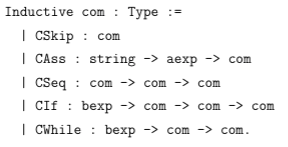
\includegraphics[scale=0.6]{ImpSyntax}
\pause
\begin{defin}[State]
A \emph{state} is a representation of \emph{all} variables at a point in time during execution of a program; variables are strings and values are in $\N$, and so formally this a (total) function from strings to naturals.  

\par Default value of ``unassigned" variables is 0.
\end{defin}
\end{frame}

\begin{frame}{The IMP language - semantics and equivalence}
Semantics of commands ($aeval$ is arithmetic evaluation, $beval$ is boolean evaluation) - note {\color{red}While rules} force termination if proof is to finish:


\noindent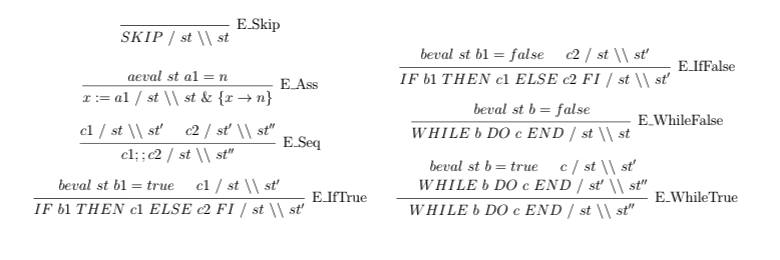
\includegraphics[scale=0.44]{ImpSemantics}
\pause
\begin{defin}[Command equivalence]
We say programs $c1$ and $c2$ are \emph{command ({\color{red} state}) equivalent} if, for all states $st$ and $st'$, $c1$ takes $st$ to $st'$ if and only if $c2$ takes $st$ to $st'$.  In Coq notation,
\[
	c1\ /\ st\ \backslash\backslash\ st' \Leftrightarrow c2\ /\ st\  \backslash\backslash\ st'.
\]
\end{defin}
\end{frame}

\begin{frame}{Opaque predicates --- command (state) equivalence} %6
\begin{defin}[Opaque predicate transformation]
An \emph{opaque predicate transformation} takes a program $c1$ and hides it behind an predicate $P$ (always true, but not obvious).
\begin{center}
IFB (P x) THEN c1 ELSE c2 FI.
\end{center} 
\end{defin}

\pause
\begin{example}
As running example, we use the (degree 2, out of range of linear SMT solvers) predicate
\[ \forall x.\ (x * x + x + x + 1) = (x + 1) * (x + 1). \]
\end{example}
 \pause
Example program: {\color{red}factorial} in IMP (input X, output Y).

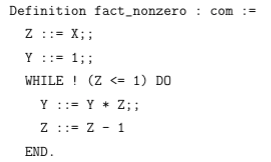
\includegraphics[scale=0.45]{factorial}
\end{frame}

\begin{frame}{Opaque predicates --- command (state) equivalence}
First attempt: define the transformation to assign value to the variable of the opaque predicate.

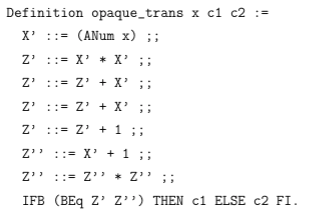
\includegraphics[scale=0.45]{opaquetrans1}
\pause\par
Able to prove both original and transformed factorial program take input $X=3$ to output $Y=6$, but...

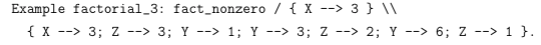
\includegraphics[scale=0.45]{fact3x1}

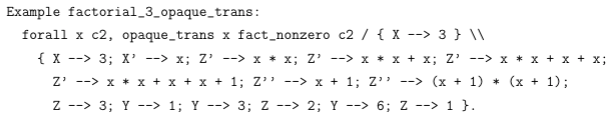
\includegraphics[scale=0.45]{fact3x2}



\end{frame}

\begin{frame}{Opaque predicates --- Hoare logic equivalence} %6

Total state equivalence (i.e.\ the value of \emph{every} variable is preserved) may be too strong of a condition and/or too much work to prove for some purposes.  Another option: \emph{Hoare logic.} \pause \medskip

\begin{defin}[Hoare triple]
	A \emph{Hoare triple}, consists of a pre-condition $P$, a program $c$, and a post-condition $Q$, written
    \[
    	(| P |)\ c\ (| Q |),
    \]
    which specifies that when $P$ is true before execution, running the program $c$ is guaranteed to make $Q$ true after execution.
\end{defin}
\pause
Proving Hoare triples in Coq is mostly mechanical, except for While loops: must find a \emph{loop invariant}.

\end{frame}

\begin{frame}{Opaque predicates --- Hoare logic equivalence}
Now only interested in a single input and single output variable, we're able to use Hoare logic to prove a more general statement.

\begin{defin}[Hoare fidelity (with respect to input X and output Y)]
A program $c_2$ preserves the {\color{red}Hoare fidelity} of a program $c_1$ with respect to input X and output Y, if the validity of the Hoare triple
\[
(| X = x_0 |)\ c_1\ (| Y = y_0 |)
\]
implies the validity of the Hoare triple
\[
(| X = x_0 |)\ c_2\ (| Y = y_0 |).
\]
\end{defin}
\pause
\begin{theo}\label{hoare_xy_main}
For all programs $c_1$ and $c_2$, and all $x \in \N$, the transformed program $opaque\_trans'(x, c_1, c_2)$ preserves the Hoare fidelity with respect to input X and output Y of $c_1$.
\end{theo}

\end{frame}

\begin{frame}{Opaque predicates -- command equivalence w/o assignment}
Revisiting command equivalence, reformulate the transformation to not assign anything and read variable values from existing state.  Allows us to prove more general theorem.

\begin{defin}
\texttt{Definition make\_opaque\_pred\_IFB b c1 c2 := IFB b THEN c1 ELSE c2 FI.}
\end{defin}
\par\medskip\pause
\begin{theo}
    If a predicate $b$ is boolean equivalent to true, then for any programs $c_1$ and c2,
the program c1 is boolean equivalent to the program resulting from applying make\_opaque\_pred
to b, c1, and c2. \par\medskip
In Coq:
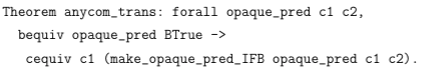
\includegraphics[scale=0.5]{anycom}


\end{theo}
    
\end{frame}

\begin{frame}{Control Flow Flattening I: Smashing Ifs}
Smashing Ifs: we turn this control flow structure
\begin{center}
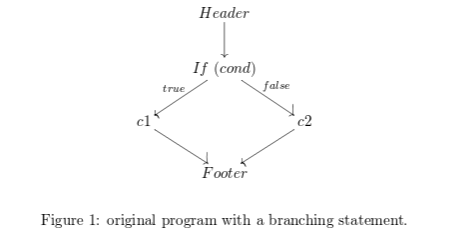
\includegraphics[scale=0.3]{IfSmash}
\end{center}
\pause \par \medskip
into this ({\color{red}augmented} IMP with Switches):
\begin{center}
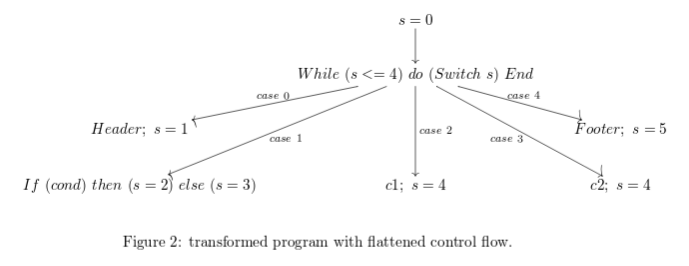
\includegraphics[scale=0.3]{IfSmash2}
\end{center}
The If-Smashing transformation takes the first (for now) If-Then construct encountered in an IMP program and transforms it into a While-Switch construct as above. 
\end{frame}

\begin{frame}{Control Flow Flattening I: Smashing Ifs}

 We want to prove: for any program $c$ (preprocessed to add $s=0$ to the start and $s=5$ to the end), it's command equivalent to applying the program we get after applying the If-Smashing algorithm to $c$.
\par\pause\medskip

Seems reasonable, right?  Should be true, right?  Ok, great, let's pack it up and ship off the product and...


\end{frame}

\begin{frame}{Control Flow Flattening I: Smashing Ifs}
...WAIT NOT SO FAST, the proof isn't going through in Coq.  What's wrong?\pause\par\medskip
Problem 1: an arbitrary program might use the switch variable used by the transformation.  So, we only want programs that don't contain the switch variable. \pause\par\medskip
Problem 2: okay, but how do you express ``the program $c$ \emph{does not} have any assignments, Ifs, or Whiles that contain the variable $s$?'' in predicate logic?  Not impossible, but way too much work and cumbersome.\pause\par\medskip
Solution: extract fundamental property that implies ``doesn't use the variable $s$" that is easy to express and work with.

\end{frame}

\begin{frame}{Control Flow Flattening I: Smashing Ifs}
\begin{defin}[Command invariance w.r.t. variable]
	For an IMP program $c$ to be \emph{command invariant} with respect to a variable $X$ means that, for all $n\in \N$, $c$ takes a state $st$ evaluates to $st'$ if and only if $c$ takes $st$ updated with $n$ assigned to $X$ to $st'$ with $n$ assigned to $X$.  In Coq notation,
    	\[
        	\forall n,\ c\ /\ st\ \backslash\backslash\ st' \Longleftrightarrow c\ /\ st\ \&\ \{ X \Rightarrow n\}\  \backslash\backslash\ st'\ \&\ \{ X \Rightarrow n\}.
        \]
\end{defin}\pause

\begin{defin}[Boolean invariance w.r.t. variable]
For a boolean statement $b$ to be \emph{boolean invariant} with respect to a variable $X$ means that for all $n\in \N$ and all states $st$, the evaluation (truth value) of $b$ in $st$ is the same as the evaluation of $b$ in $st$ with $n$ assigned to $X$; in Coq notation,
\[
	\forall n,\ st,\ beval\ b\ st\  = beval\ b\ st\ \&\ \{ X \Rightarrow n\}.
\]
\end{defin}
\end{frame}

\begin{frame}{Control Flow Flattening I: Smashing Ifs}
\begin{theo}
Let $s$ be a switch variable.  Any program $c$ in the form
\begin{align*}
	c =&\ s ::= 0 \\
    &\ header \\
    &\ IFB\ (cond)\ THEN\ (c1)\ ELSE\ (c2)\ FI \\
    &\ footer \\
    &\ s ::= 5 
\end{align*}
       is command equivalent to the $If-Smash$ transformed version of $c$ if:
       \begin{itemize}
       		\item $c1$ and $c2$ are command invariant with respect to $s$.
            \item $cond$ is boolean invariant with respect to s.
       \end{itemize}
\begin{proof}
	Done in Coq.  Long, but many parts mechanical.  Need to invoke Law of Excluded Middle to do case analysis on truth values and invoke determinism of command eval (a separate intermediary theorem).
\end{proof}
\end{theo}
\end{frame}

\begin{frame}{Control Flow Flattening I: Smashing Ifs}
Takeaways:
\begin{itemize}
	\item It's easy to make a statement or argument that ``sounds about right'' but overlook details that could cause catastrophic problems down the line. \pause
    \item Formal verification not only proves the thing does as it says, but allows you to catch bugs \emph{before} they even become code. \pause
    \item We've just ``tested" (proven) that our toy transformation works correctly on an infinite class of programs that satisfies a few simple conditions!\pause
    \item Something something prevention, something something cure.
\end{itemize}

\end{frame}

\begin{frame}{Control Flow Flattening II: Smashing Whiles}
Two ways to transform While statements.  \par First method: turn it into a If-then-goto (call this ``dismantling").
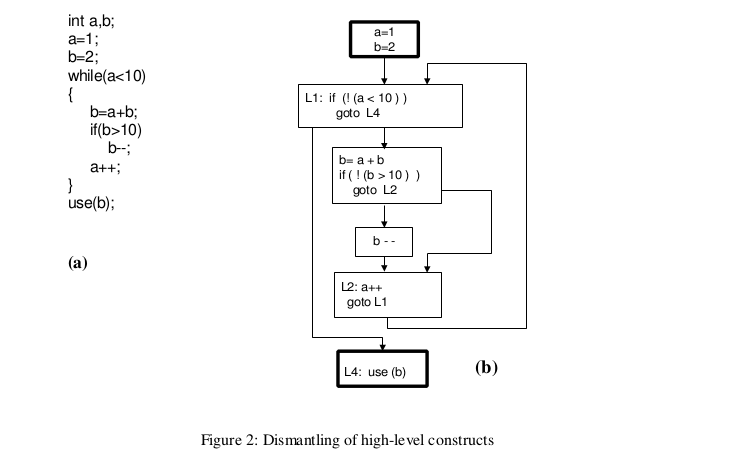
\includegraphics[scale=0.4]{WhileSmash}\par
(Diagram taken from paper by Chenxi Wang et al.)
\end{frame}


\begin{frame}{Control Flow Flattening II: Smashing Whiles}
Second method: turn it into a switch (call this ``flattening'' proper).
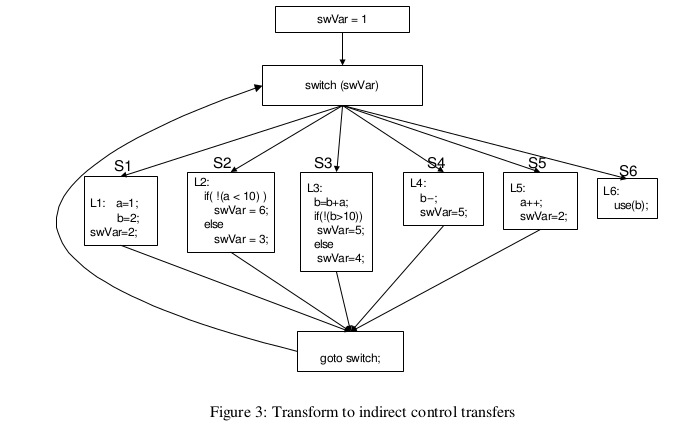
\includegraphics[scale=0.4]{WhileSmash2}\par
(Diagram taken from paper by Chenxi Wang et al.)
\end{frame}

\begin{frame}{Control Flow Flattening II: Smashing Whiles}
Define a new ImpFlow language, wrapping up blocks of code with instructions on which block to go to next.  Syntax:

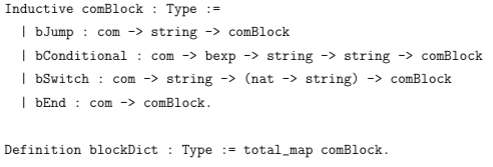
\includegraphics[scale=0.6]{ImpFlow}
\pause
Program definitions get long and unwieldy, not practical to put on slides.  Lower-level.  But representation of real-life tools (eg Cloakware) which will transpile to lower-level intermediate languages for part of obfuscation.
\pause\par\medskip

Proved: example in Coq modelling diagrams on previous slides.  Original, dismantled, and flattened version of the same program take input $A=1, B=2$ to $RETURN=12$.


\end{frame}

\begin{frame}{Related works}
    Three papers by Sandrine Blazy et al.
    \begin{itemize}
        \item 2012 paper also uses IMP, studies data obfuscation techniques (as opposed to our layout techniques): \emph{distorted semantics} (map from $\N$ to $\N$ and \emph{variable encoding}.  Different class of obfuscations.
        \item 2016 paper studies control flow flattening in CompCert instead of IMP.  Goes through intermediate language CLight.  Rest of compilation process ``free" from CompCert's own proofs.
        \item 2019 paper continues in CLight: mixed boolean-arithmetic expressions (mix arithmetic operations with bitwise boolean operations).  Beyond scope of present discussion.
    \end{itemize}
\end{frame}

\begin{frame}{Future directions}
    \begin{itemize}
        \item Different levels of languages: IMP to CompCert.  Simple and theoretical vs complex and practical.  Value in both.
        \item Combine different obfuscation proofs together, since real world tools will use many disparate transformations at once.
        \item Other properties of interest: transformation should be \emph{small} and \emph{efficient} (polynomial bounds on size and performance).
        \item Other properties of interest: security properties.  Formulating the correct thing to prove in itself is a challenge.  (Impossibility result for strongest \emph{virtual black box} - oracle vs source access - condition).
    \end{itemize}
\end{frame}

\begin{frame}{The end.}
\begin{center}\medskip

\includegraphics[]{thanks}
\end{center}
Thanks to:
\begin{itemize}
\item Profs Phil Scott and Amy Felty for the supervision.
\item Profs GV Jourdan, Luigi Logrippo, and Liam Peyton for being on the committee.
\item Dr Bahman Sistany (Irdeto) for the summer work term where this began.
\item OGS and uOttawa for financial support.
\end{itemize}
\end{frame}

\end{document}
